\documentclass[11pt]{article}

\usepackage[margin=1in]{geometry}
\usepackage{amsmath,amssymb}
\usepackage{booktabs}
\usepackage{graphicx}
\usepackage{subcaption}
\usepackage{hyperref}

\graphicspath{{images/}}
\hypersetup{
  colorlinks=true,
  linkcolor=blue,
  urlcolor=blue,
  citecolor=blue
}

\title{CS728 Programming Assignment 3}
\author{Kshitij Vaidya (22B1829), Jay Mehta (22B1281), Tanay Bhat (22B3303)}

\begin{document}
\maketitle
\section{Part 1: Classical Retrieval}
\subsection{Comparison of Retrieval Methods}
\begin{table}[ht]
\centering
\begin{tabular}{ccc}
\toprule
\textbf{Method} & \textbf{Recall@1} & \textbf{Recall@5} \\

\midrule
\textbf{BM25} & 0.2312 & 0.4114 \\
\textbf{msmarco-MiniLM} & 0.3882 & 0.6106 \\
\textbf{UAE-large-v1} & 0.6502 & 0.8842 \\
\bottomrule
\end{tabular}
\caption{Recall at different ranks for the three retrieval methods.}
\label{tab:recall}
\end{table}

\section{Part 2: Lost-in-the-middle}
\subsection{Results}
\begin{itemize}
    \item Recall@1: 0.0122
    \item Recall@5: 0.2486
\end{itemize}
\subsection{Plot}
\begin{figure}
    \centering
    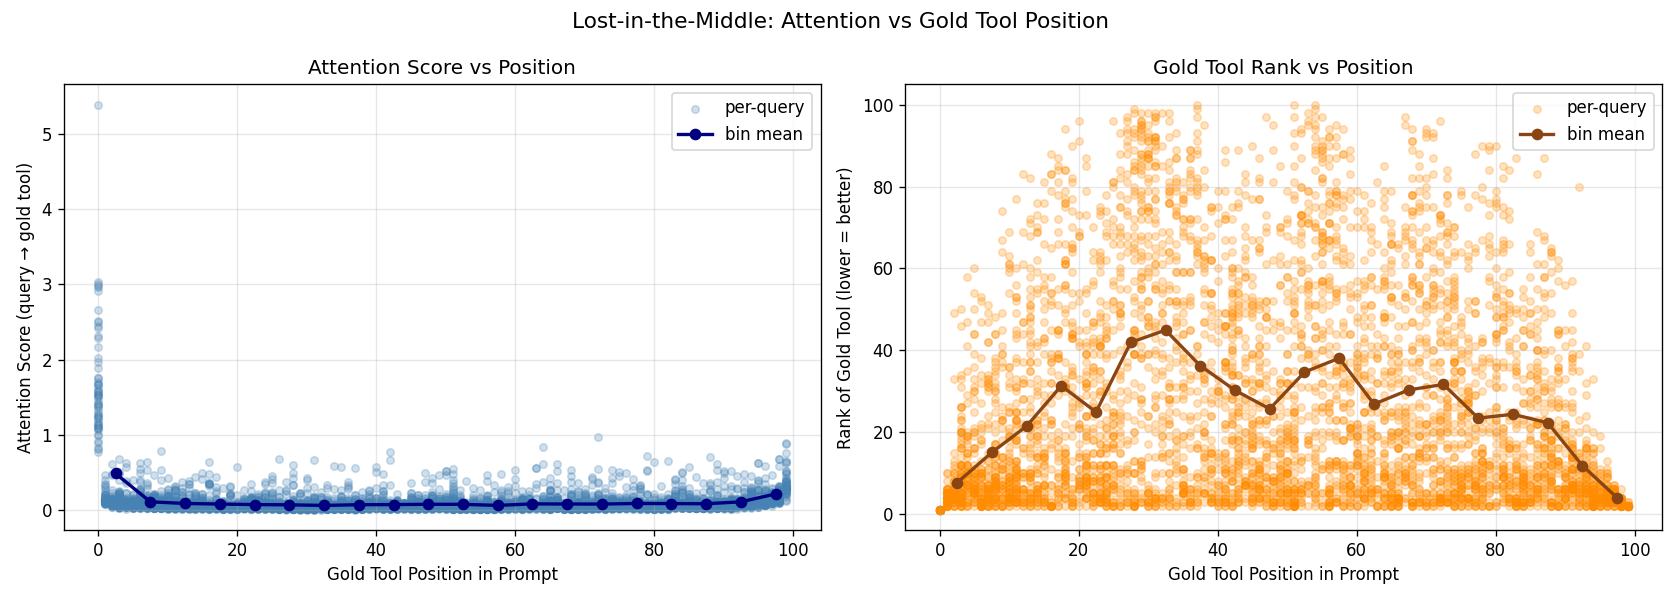
\includegraphics[width=0.8\textwidth]{../gold_attention_plot.png}
    \caption{Position Effect on Attention Based Ranking}
    \label{fig:recall_plot}
\end{figure}
\section{Part 3: Retrieval Heads}
\subsection{Head selection strategy}
TO-DO

\textbf{Selected Heads:}
[(6, 11), (7, 12), (4, 16), (5, 11), (8, 19), (10, 9), (2, 20), (10, 1), (6, 8), (10, 23), (6, 9), (5, 10), (8, 20), (8, 13), (12, 13), (5, 9), (10, 13), (10, 11), (8, 17), (10, 26)]

\small{Note: format of selected heads is (layer number, head number).}


\subsection{Results}
\begin{itemize}
    \item Recall@1: 0.2632
    \item Recall@5: 0.5918
\end{itemize}

\subsection{Comparison with previous methods}


\end{document}
